\begin{quote}
	\textit{``The major challenge for the future will be effectively and cheaply to shift the sense of presence from one's own body to another, without replacing or excluding the physical world in which we all exist.''}
\end{quote}
\hfill \textit{Distributed Embodiment: Real Presence in Virtual Bodies, Waterworth \& Waterworth}
\\
\\
%=========================================================================================================
%=========================================================================================================

\label{introduction}

%=========================================================================================================

A tourist steps into a 15th century chapel. Although the chapel is in remarkable condition for a building that is over 500 years old (it is even still in active use!) it looks markedly different today than it did when it was first built, back in 1450. The tourist dons a head-mounted display, which via a pair of front mounted cameras allows her to still see where she is going as she starts to explore the chapel. Once in the centre of the building, she stops walking \& presses a button on a controller in her hand. Her view of the chapel around her disappears \& is replaced with a virtual reconstruction of the chapel as it stood over 500 years ago. The view changes appropriately as she turns her head, allowing her to look all around her at how chapel used to be. She releases the button \& is returned to the present day \& continues walking through the chapel until she reaches the altar. She presses the button again \& once again her view switches to that of the virtual chapel, which has moved to match her new position at the altar, allowing her to inspect its 1450 counterpart.

This is not an augmented reality system which superimposes virtual objects upon the real world. This is a \textbf{parallel reality} system that allows its user to switch between seeing the real world \& a complete, immersive virtual environment, allowing access to a level of tandem virtuality unprecedented of augmentations.

\afterpage{
\begin{figure}[h]
	\begin{center}
	   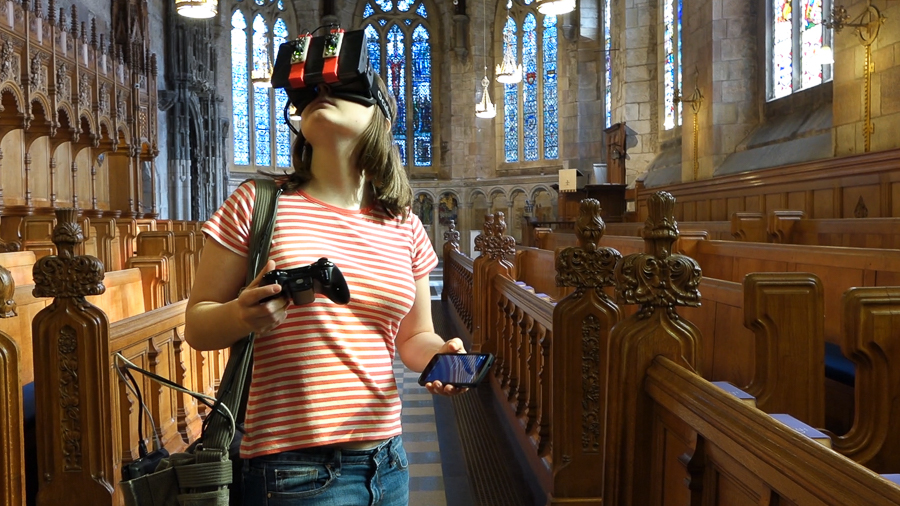
\includegraphics[width=\textwidth]{participant-f-2.jpg}
	\end{center}
	\label{participant-f-2.jpg}
	\caption{The \textit{Mirrorshades} parallel reality platform in use at a 15th century chapel. This image is taken from a video that is available to view online\protect\footnotemark .}
\end{figure}

\footnotetext{\url{https://www.youtube.com/watch?v=UsDRPjDwr8A}}
}

%=========================================================================================================

\section{Parallel Reality}

The central theme of this thesis is the concept of `parallel reality', defined thus;

\vspace{7mm}

\textbf{Parallel Reality:} A system comprising two environments, one real \& the other virtual, wherein each is complete unto itself \& the user may freely move between the two.

\vspace{7mm}




background of alternate realities, cross reality, the vacancy problem, the opening Waterworth quote, introducing parallel reality as the next step/solution, etc.

%=========================================================================================================

\section{Contributions}

The contributions of this thesis can be summarized as follows;

\begin{itemize}
	\item The introduction of parallel reality as a new category of alternate reality that allows users to experience two complete environments in tandem \& represents a solution for mitigation of the vacancy problem.
	\item The framing of parallel reality through a thorough investigation \& extension of previous taxonomies that classify \& distinguish alternate reality terms.
	\item The creation of the combined Milgram/Waterworth model for visualising alternate realities experiences, including parallel reality.
	\item Development of a parallel reality platform, dubbed Mirrorshades, that combines new virtual reality hardware with novel indoor positioning technology.
	\item Evaluation of the Mirrorshades platform through user studies of a real world use case within the realm of cultural heritage, including the application of an established presence questionnaire to parallel reality.
	\item Discussion \& creation of a set of best practices for future parallel reality endeavours.
\end{itemize}

%=========================================================================================================

\section{Research Domains}

alternate realities, virtual reality, digital/virtual heritage
imaging
presence, psychology, experience
indoor positioning

%=========================================================================================================

\section{Document Overview}

Chapter \ref{chapter-background} surveys existing taxonomies \& methods for classifying, categorising \& distinguishing between different alternate reality techniques, in order to frame the introduction of the parallel reality concept against existing techniques. Chapter \ref{chapter-vtw} describes the development of an initial tablet based parallel reality system while chapter \ref{chapter-mirrorshades} details the development of the Mirrorshades parallel reality platform. Chapters \ref{chapter-eval-1} \& \ref{chapter-eval-2} cover the evaluation of the Mirrorshades platform through user studies at a cultural heritage site, the former comparing parallel reality against more traditional manners in which virtual reality are used at such sites \& the latter investigating the benefits \& drawbacks to manners of parallel reality implementation, presenting a set of best practice recommendations. Finally \ref{chapter-conclusions} concludes the body of work \& postulates on future avenues of parallel reality investigation.

%=========================================================================================================

















%=========================================================================================================

The concept of alternate realities that is popularly held today has become a mainstay both of science fiction \& of serious academic research, with the concept of other worlds \& how we can visit them or bring them into our `real' world keeping authors \& scientists alike fascinated for many decades. The concept of these `virtual worlds' dates back far into human history, long before mankind's invention of the transistor \& the computers that followed it;

\begin{quote}
	\textit{``Virtual worlds, or as we will now ore broadly define them, immersive experiences delivered through the human imagination, have their origins in deep prehistory. Whether these varieties of nonphysical, dreamlike realities were communicated by our ancestors through the imitation of animals, the incarnation of spirits, the painting of scenes on the stone canvasses of caves, the holding of ceremonial rites in temples, or the elaboration of the human story through the fount of theater, humans have craved and crafted virtual-world experiences from the dawn of artistic and linguistic expression.''}~\cite{Damer2014}
\end{quote}

However within this thesis we are concerned with alternate realities as those that through means of computer modify, mediate or create the environmental stimuli that reach a subject's senses.

While some alternate reality endeavours have explored the mediation of multiple human senses, from Morton Heilig's 1950's `Sensorama' experience that presented its occupant with a motorcyle ride through combination of film, sound, wind, vibration \& odor~\cite{Rheingold1992}, to present day experiences that combine multiple computer generated sensory data such as the Birdly full body flight simulator\footnote{\url{http://birdly.zhdk.ch/}}, many are focussed for good reason upon visual stimuli alone;

\begin{quote}
	\textit{``Sight plays such a prominent part in the mental life that the field of vision is sometimes considered almost synonymous with the field of attention.''}~\cite{Lucas1951}
\end{quote}

The 1990s saw a surge of interest around \textit{virtual reality}, promising via head mounted displays to immerse users into 3D virtual environments. However with hardware \& software simply not advanced enough to meet the hype, the virtual reality bubble burst \& was largely ignored as a consumer platform for gaming \& media consumption.

The advent \& mass adoption of the smartphone beginning in the early 2000s, with its combination of location sensing (GPS) \& orientation sensing (accelerometer \& gyroscope) capabilities in a portable package with a screen \& camera, led to a surge of \textit{augmented reality} applications, which would overlay virtual objects \& data upon a view of the real world seen through the phone's camera.


3D3C virtual worlds such as Second Life

led to a flurry of interesting research that
vacancy problem
polysocial reality, wanting to be in both real \& virtual

the Oculus Rift of the early 2010s



Then leading to my research, parallel reality




From William Gibson's `The Gernsback Continuum' \& beyond through contemporary cyberpunk literature

the `gargoyles' of MIT

``the reality games of Philip K Dick''~\cite{Sterling1988} \& the almost constant virtual overlays of the real world described in Vernor Vinge's Rainbows End~\cite{Vinge2006}






And the Media Lab invented what they would call Cross Reality that linked a real world location with a virtual other via sensors \& actuators, such that an inhabitant of one could glimpse a tantalizing insight into the goings on of the `other' although they could not see into it.

This thesis explores an alternate reality that as yet has received little attention or even a name. Parallel Reality as it came to be called builds upon the concept of Cross Reality \& its two distinct environments each `complete unto itself'. But instead of the shadow of one environment only laying upon the other by manner of sensors \& actuators, new VR technology combined with indoor positioning systems allow a user to switch between environments - to at one moment view their RW surroundings \& at the next to view the equivalent vantage in a parallel virtual environment

%=====================
%On why alternate realities are predominantly visual?

\textit{``visual ordination of intellectual knowledge''}

\textit{``Seeing remains an insistent metaphor for all of cognition only because while the ocular lobes are merely one of our brain's tentacular connections to reality, they are among the most `conscious' of their capacity for information control.''}

The Mediated Sensorium, Caroline A. Jones




Into background chapter

\textit{``virtual reality is a technology that convinces the participant that he or she is actually in another place by substituting the primary sensory input with data received produced by a computer''}~\cite{Heim1998}


%=====================


%can sound alone give us an alternate reality?
Caroline A. James speaking on the work of Janet Cardiff \& George Bures Miller
\textit{``Cardiff brings segmentation into the present, crafting `sound walks' that layer an alternate reality over the fl\^aneur's perambulations - a fantastic elaboration of the kind of personal soundscape chosen by the iPod user.''}

%=========================================================================================================